\section{Observer}

O padrão Observer permite criar uma dependência de muitos 
objetos para um entre objetos. Dessa forma, quando um 
objeto em específico é alterado, um grupo de objetos 
pré-configurados é notificado. Esse comportamento é 
semelhante a um \textit{publish and subscribe}, onde 
um objeto é um \textit{publisher} que publica notificações 
para os objetos inscritos. A dinâmica do padrão pode ser 
vista no diagrama da figura \ref{observer_struct}.

\begin{figure}[htb]
	\caption{\label{observer_struct}Estrutura do Observer}
	\begin{center}
	    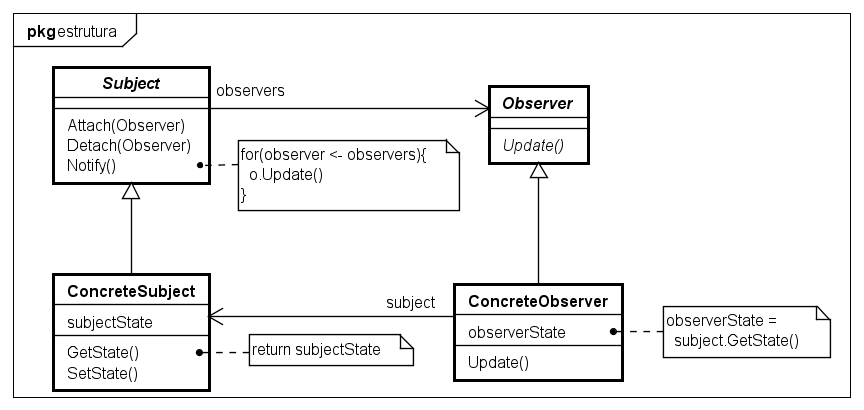
\includegraphics[scale=0.5]{5_padroes-contexto-funcional/5.3_comportamentais/5.3.07_observer/observer_estrutura.png}
	\end{center}
\end{figure}

\subsection*{Exemplo Orientado a Objetos}

Como exemplo, pode ser considerada uma aplicação 
gráfica que possui uma tabela e um gráfico de 
barras que apresentam informações de grupos 
A, B e C. Essas informações são dados utilizados 
pela aplicação que podem ser alterados por outros 
elementos gráficos, como botões ou caixas de texto. 
Para que a tabela e o gráfico estejam atualizados, 
eles são armazenados pela classe que centraliza 
esses dados de forma que ela os notifique 
caso os dados sejam atualizados. O diagrama 
de classes para o exemplo pode ser visto na figura 
\ref{observer_exemplo}, enquanto a implementação 
pode ser vista no código \ref{ooobserver}.

\begin{figure}[htb]
	\caption{\label{observer_exemplo}Exemplo de Observer}
	\begin{center}
	    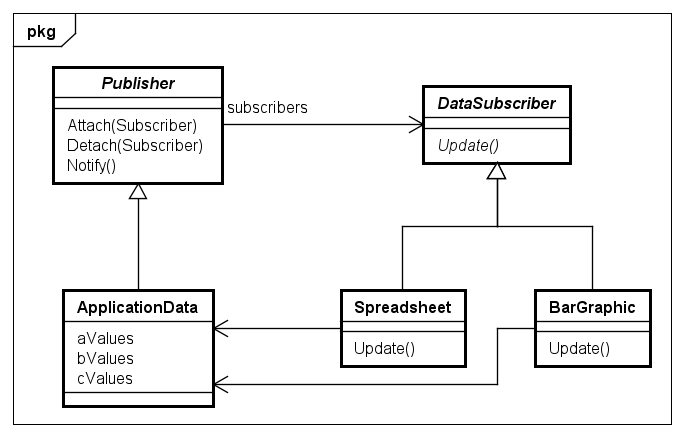
\includegraphics[scale=0.5]{5_padroes-contexto-funcional/5.3_comportamentais/5.3.07_observer/observer_exemplo.png}
	\end{center}
\end{figure}

\begin{lstlisting}[caption={Observer Orientação a Objetos},label=ooobserver]

abstract class Publisher {
  private var subscribers : List[DataSubscriber] = List.empty

  def Attach(subscriber: DataSubscriber) : Unit = {
    subscribers = subscriber :: subscribers
  }

  def Detach(subscriber: DataSubscriber) : Unit = {
    subscribers = subscribers.filter(sub => sub != subscriber)
  }

  def Notify() : Unit = {
    for(subscriber <- subscribers){
      subscriber.Update()
    }
  }
}

class ApplicationData extends Publisher {
  private var aValues : List[Int] = List.empty
  private var bValues : List[Int] = List.empty
  private var cValues : List[Int] = List.empty

  def SetValues(_aValues : List[Int],
                _bValues : List[Int],
                _cValues : List[Int]): Unit = {
    this.aValues = _aValues
    this.bValues = _bValues
    this.cValues = _cValues
    Notify()
  }

  def GetAValues() : List[Int] = aValues
  def GetBValues() : List[Int] = bValues
  def GetCValues() : List[Int] = cValues
}

trait DataSubscriber {
  def Update()
}

class Spreadsheet(val data : ApplicationData) extends DataSubscriber {
  override def Update(): Unit = {
    var aValues = data.GetAValues()
    var bValues = data.GetBValues()
    var cValues = data.GetCValues()
    //Atualiza a tabela com os novos valores
  }
}

class BarGraphic(data: ApplicationData) extends DataSubscriber {
  override def Update(): Unit = {
    var aBar = data.GetAValues().sum
    var bBar = data.GetBValues().sum
    var cBar = data.GetCValues().sum
    //Atualiza o gráfico com os novos valores
  }
}
    
\end{lstlisting}

\subsection*{Contexto Funcional}

O padrão Observer depende bastante de 
efeitos colaterais em sua implementação, 
já que depende de outros objetos serem avisados 
quando o estado do objeto observado for 
atualizado. Uma abordagem semelhante à vista 
no padrão Mediator, onde as funções clientes 
gerenciam os observáveis e os subordinados, 
poderia ser utilizada para trazer um resultado 
semelhante. Porém, existe uma abordagem - a 
programação reativa funcional - que se encaixa 
no contexto funcional e serve como alternativa 
para o padrão Observer\cite{reactiveprog}.

Programação reativa funcional pode ser entendida 
como a interseção entre programação reativa e 
programação funcional. Programação reativa traz a 
ideia de reagir ou responder a eventos, que são 
mensagens propagadas por um programa. Dessa forma, 
programação reativa funcional é um método de 
programação reativa que busca aproveitar os 
conceitos de composicionalidade e funções puras 
da programação funcional.\cite{reactiveprog}
\footnote{A linguagem Scala suporta programação 
reativa funcional através do \textit{framework} 
Akka, disponível em \url{https://akka.io/}.}